    Ejercicio 8. Un profesor califica a sus alumnos según el criterio siguiente: 40\% de suspensos, 30\% de aprobados, 15\% notables, 10\% sobresalientes y 5\% de matrículas. Las notas obtenidas son las siguientes: \\
    
    \begin{tabular}{| c | c | c | c | c | c | c | c | c | c |}
        \hline
        (0,1] & (1,2] & (2,3] & (3,4] & (4,5] & (5,6] & (6,7] & (7,8] & (8,9] & (9,10] \\ \hline
        34 & 74 & 56 & 81 & 94 & 70 & 41 & 28 & 16 & 4 \\ \hline
    \end{tabular} \\
    
    Calcular las notas máximas para obtener cada una de las calificaciones. 
    \\
    \\
    POBLACIÓN: Los alumnos. \\
    TAMAÑO: $34+74+56+81+94+70+41+28+16+4=498$ \\
    MODALIDADES: Los intervalos que contienen las notas obtenidas en los exámenes. \\
    
    \begin{center}
    \begin{tabular}{| c | c | c | c | c |}
        \hline
        $x_i$ & $n_i$ & $N_i$ & $f_i$ & $F_i$ \\ \hline
        (0,1] & 34 & 34 & $\frac{34}{498}$ & $\frac{34}{498}$ \\
        (1,2] & 74 & 108 & $\frac{74}{498}$ & $\frac{108}{498}$ \\
        (2,3] & 56 & 164 & $\frac{56}{498}$ & $\frac{164}{498}$ \\
        (3,4] & 81 & 245 & $\frac{81}{498}$ & $\frac{245}{498}$ \\
        (4,5] & 94 & 339 & $\frac{94}{498}$ & $\frac{339}{498}$ \\
        (5,6] & 70 & 409 & $\frac{70}{498}$ & $\frac{409}{498}$\\
        (6,7] & 41 & 450 & $\frac{41}{498}$ & $\frac{450}{498}$\\
        (7,8] & 28 & 478 & $\frac{28}{498}$ & $\frac{478}{498}$\\
        (8,9] & 16 & 494 & $\frac{16}{498}$ & $\frac{494}{498}$\\
        (9,10] & 4 & 498 & $\frac{4}{498}$ & 1 \\ \hline
    \end{tabular}
    \end{center}
    
    \begin{center}
    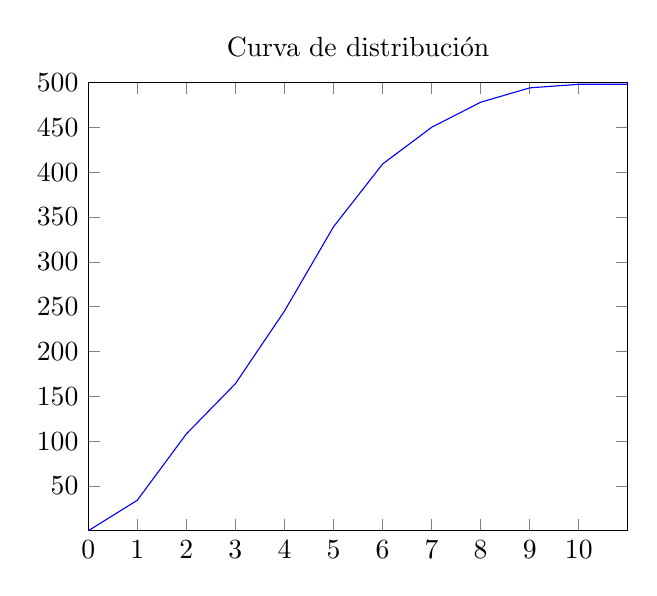
\begin{tikzpicture}
    \begin{axis}[
        title={Curva de distribución},
        xmin=0, xmax=11,
        ymin=0, ymax=500,
        xtick={0,1,2,3,4,5,6,7,8,9,10},
        ytick={50,100,150,200,250,300,350,400,450,500},
        legend pos=north west,
        ymajorgrids=false,
        grid style=dashed,
    ]

    \addplot[
        color=blue,
        ]
        coordinates {
        (0,0)(1,34)(2,108)(3,164)(4,245)(5,339)(6,409)(7,450)(8,478)(9,494)(10,498)(11,498)
        };
    
    \end{axis}
    \end{tikzpicture}
    \end{center} 
    Para la curva de distribución, en el eje x tenemos los extremos de los intervalos y en el eje y ponemos $N_i$, la frecuencia absoluta acumulada. \\ \\
    Para hallar las notas máximas para obtener cada una de las calificaciones calculamos los percentiles. La nota que fuese el percentil 30, por ejemplo, significa que el 30\% de la población, tiene una nota igual o menor a ella, es decir, un suspenso en este caso. \\ \\ 
    Empezamos calculando la nota máxima para sacar un suspenso. Como el 40\% son suspendidos, calculamos el percentil 40, o lo que es lo mismo, el decil 4. $P_{40} = D_{4} = \frac{nr}{100} = \frac{498*40}{100} = 199.2$. Vemos en la tabla que en la columna de la frecuencia absoluta acumulada, $N_4$ es la inmediatamente mayor a 199.2. Así sabemos que el percentil 40 va a estar en el intervalo $I_4 = (3,4]$. Vamos a la curva de distribución y hacemos semejanza de triángulos. \\
    
    \begin{center}
    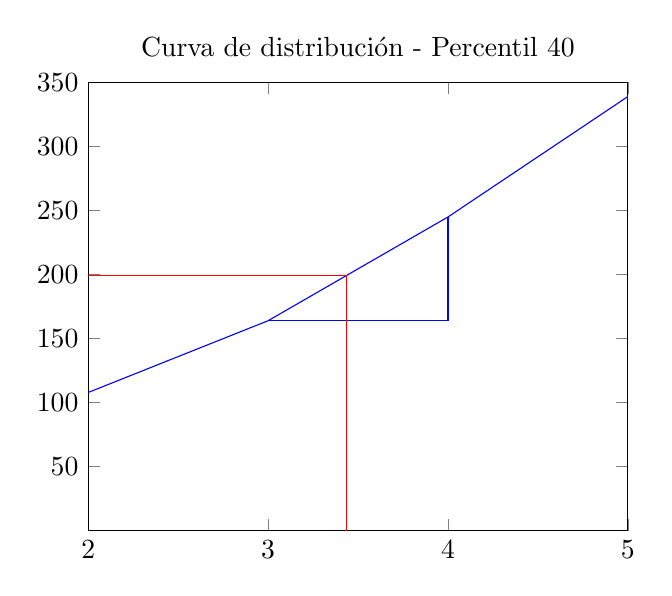
\begin{tikzpicture}
    \begin{axis}[
        title={Curva de distribución - Percentil 40},
        xmin=2, xmax=5,
        ymin=0, ymax=350,
        xtick={2,3,4,5},
        ytick={50,100,150,200,250,300,350},
        legend pos=north west,
        ymajorgrids=false,
        grid style=dashed,
    ]

    \addplot[
        color=blue,
        ]
        coordinates {
        (2,108)(3,164)(4,245)(5,339)
        };
    \addplot[
        color=blue,
        ]
        coordinates {
        (3,164)(4,164)(4,245)
        };
    \addplot[
        color=red,
        ]
        coordinates {
        (2,199.2)(3.435,199.2)(3.435,0)
        };
    
    \end{axis}
    \end{tikzpicture}
    \end{center} 
    Hacemos $\frac{P_{40}-3}{4-3}=\frac{199.2-164}{245-164}$. Así obtenemos que $P_{40} = 3.435$. Esto es que el 40\% de la población tiene una nota inferior a esta, un 3.435 es la máxima nota dentro de los suspensos. \\ \\
    Para los aprobados, tenemos que buscar una nota tal que por debajo de ella estén todos los aprobados y los suspendidos, es decir, $30+40 = P_{70}$. De nuevo hacemos $P_{70}=D_{7}=\frac{498*70}{100}=348.6$. Vemos en la tabla que $N_{6}$ es la inmediatamente mayor a 348.6. El percentil 70 está en el intervalo $I_6 = (5,6]$. Vamos a la curva de distribución y hacemos semejanza de triángulos. \\
    
    \begin{center}
    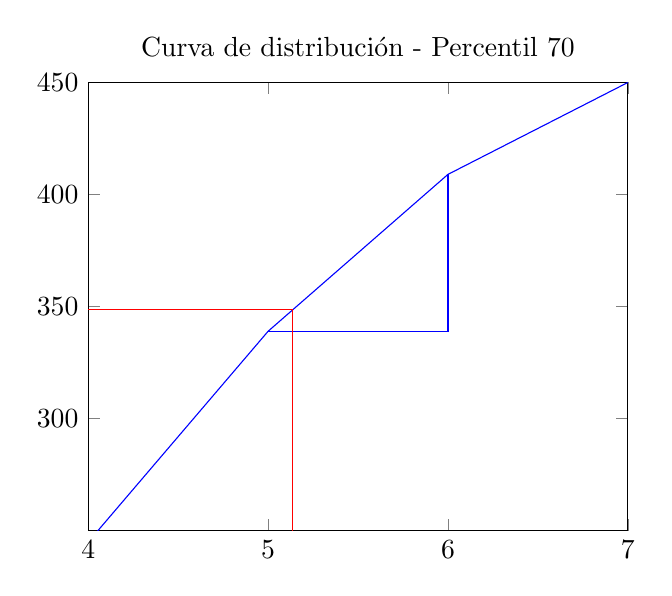
\begin{tikzpicture}
    \begin{axis}[
        title={Curva de distribución - Percentil 70},
        xmin=4, xmax=7,
        ymin=250, ymax=450,
        xtick={4,5,6,7},
        ytick={300,350,400,450},
        legend pos=north west,
        ymajorgrids=false,
        grid style=dashed,
    ]

    \addplot[
        color=blue,
        ]
        coordinates {
        (4,245)(5,339)(6,409)(7,450)
        };
    \addplot[
        color=blue,
        ]
        coordinates {
        (5,339)(6,339)(6,409)
        };
    \addplot[
        color=red,
        ]
        coordinates {
        (2,348.6)(5.137,348.6)(5.137,0)
        };
    
    \end{axis}
    \end{tikzpicture}
    \end{center} 
    Hacemos $\frac{P_{70}-5}{6-5}=\frac{348.6-339}{409-339}$. Así obtenemos que $P_{70} = 5.137$. Esto es que el 70\% de la población tiene una nota inferior a esta, de los cuales un 40\% son suspensos. Un 5.137 es la máxima nota para un aprobado. \\ \\
    Para los notables, tenemos que buscar una nota tal que por debajo de ella estén todos los notables, aprobados y suspendidos, es decir, $30+40+15 = P_{85}$. De nuevo hacemos $P_{85}=\frac{498*85}{100}=423.3$. Vemos en la tabla que $N_{7}$ es la inmediatamente mayor a 423.3. El percentil 85 está en el intervalo $I_7 = (6,7]$. Vamos a la curva de distribución y hacemos semejanza de triángulos. \\
    
    \begin{center}
    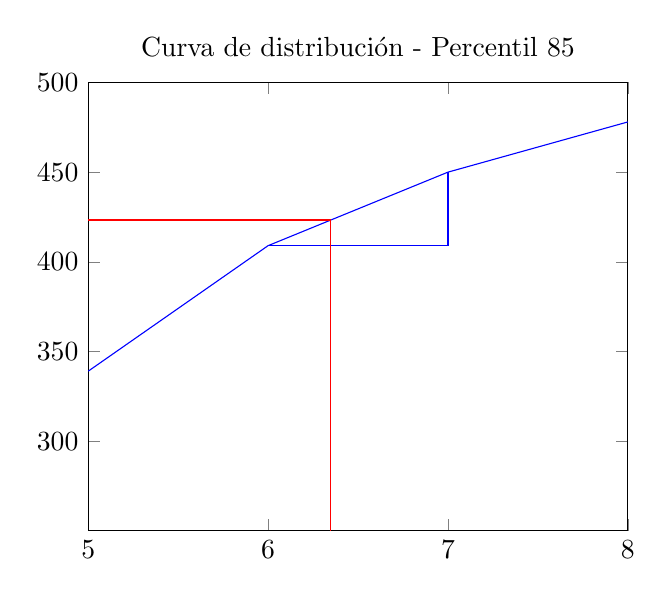
\begin{tikzpicture}
    \begin{axis}[
        title={Curva de distribución - Percentil 85},
        xmin=5, xmax=8,
        ymin=250, ymax=500,
        xtick={5,6,7,8},
        ytick={300,350,400,450,500},
        legend pos=north west,
        ymajorgrids=false,
        grid style=dashed,
    ]

    \addplot[
        color=blue,
        ]
        coordinates {
        (5,339)(6,409)(7,450)(8,478)
        };
    \addplot[
        color=blue,
        ]
        coordinates {
        (6,409)(7,409)(7,450)
        };
    \addplot[
        color=red,
        ]
        coordinates {
        (5,423.3)(6.349,423.3)(6.349,0)
        };
    
    \end{axis}
    \end{tikzpicture}
    \end{center} 
    Hacemos $\frac{P_{85}-6}{7-6}=\frac{423.3-409}{450-409}$. Así obtenemos que $P_{85} = 6.349$. Esto es que el 85\% de la población tiene una nota inferior a esta, de los cuales un 40\% son suspensos y un 30\% aprobados. Un 6.349 es la máxima nota para un notable. \\ \\
    Para los sobresalientes, tenemos que buscar una nota tal que por debajo de ella estén todos los sobresalientes, notables, aprobados y suspendidos, es decir, $30+40+15+10 = P_{95}$. De nuevo hacemos $P_{95}=\frac{498*95}{100}=473.1$. Vemos en la tabla que $N_{8}$ es la inmediatamente mayor a 473.1. El percentil 95 está en el intervalo $I_8 = (7,8]$. Vamos a la curva de distribución y hacemos semejanza de triángulos. \\
    
    \begin{center}
    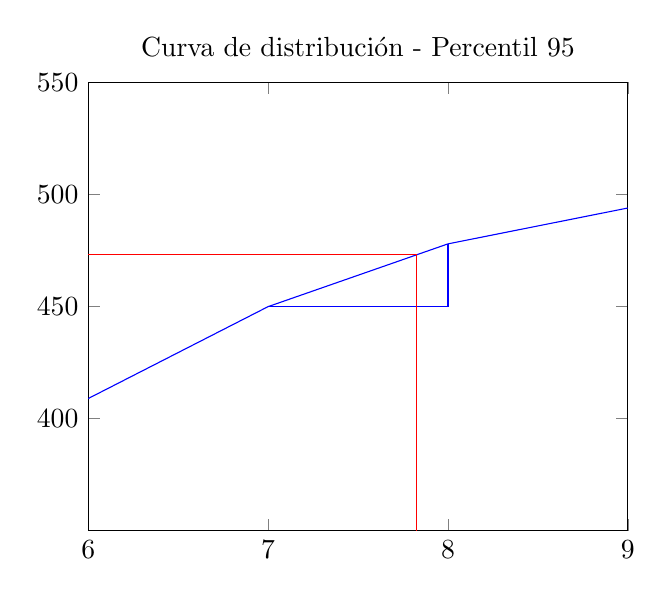
\begin{tikzpicture}
    \begin{axis}[
        title={Curva de distribución - Percentil 95},
        xmin=6, xmax=9,
        ymin=350, ymax=550,
        xtick={6,7,8,9},
        ytick={400,450,500,550},
        legend pos=north west,
        ymajorgrids=false,
        grid style=dashed,
    ]

    \addplot[
        color=blue,
        ]
        coordinates {
        (6,409)(7,450)(8,478)(9,494)
        };
    \addplot[
        color=blue,
        ]
        coordinates {
        (7,450)(8,450)(8,478)
        };
    \addplot[
        color=red,
        ]
        coordinates {
        (6,473.1)(7.825,473.1)(7.825,0)
        };
    
    \end{axis}
    \end{tikzpicture}
    \end{center} 
    
    Hacemos $\frac{P_{95}-7}{8-7}=\frac{473.1-450}{478-450}$. Así obtenemos que $P_{95} = 7.825$. Esto es que el 95\% de la población tiene una nota inferior a esta, de los cuales un 40\% son suspensos, un 30\% aprobados y un 10\% notables. Un 7.825 es la máxima nota para un sobresaliente. \\ \\
    Para las matrículas, tenemos que buscar una nota tal que por debajo de ella estén todas las matrículas, sobresalientes, notables, aprobados y suspendidos, es decir, todas las notas, $30+40+15+10+5 = 100 = P_{100}$. Hacemos $P_{100}=\frac{498*100}{100}=498$. Vemos en la tabla que $N_{10}$ es 498. Un 10 es la máxima nota para una matrícula.